\documentclass[]{article}
\usepackage[utf8]{inputenc}
\usepackage[]{graphicx}
\usepackage{geometry}
\usepackage{listings}

%\geometry{tmargin=0.5cm,bmargin=0.5cm,lmargin=0.5cm,rmargin=0.5cm}
\title{PREPROYECTO ENTREGA 2 MODELO RELACIONAL , ENTIDAD RELACIÓN , DDL  Y CONSULTAS BÁSICAS EN SQL. }
\author{\textbf{Luis Felipe Vargas Rojas}  \emph{código 0836342} \\
         \textbf {Edgar Andres Moncada} \emph{ código 0832294} }
\begin{document}
\newpage
\maketitle
\section{Bocetos De Interfaz.}

\begin{figure}[h]
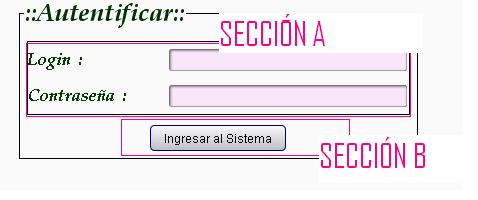
\includegraphics[width= 10cm , height= 5cm]{Bocetos/AUTENTICAR.jpg}
\caption{Boceto De interfaz Autenticar usuario , la cual permite ingresar al sistema como usuario con ciertos privilegios.}
\end{figure}

\begin{figure}[h]
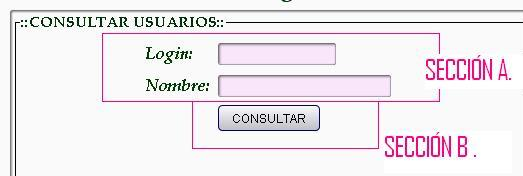
\includegraphics[width= 10cm , height= 5cm,angle=0]{Bocetos/consultarUsuarios.jpg}
\caption{Boceto De Interfaz  Consultar Usuarios La Cual Permite Al Administrador Consultar Los Usuarios De La Base De Datos y Modificar Algunos Datos De Este. }
\end{figure}

\begin{figure}[h]
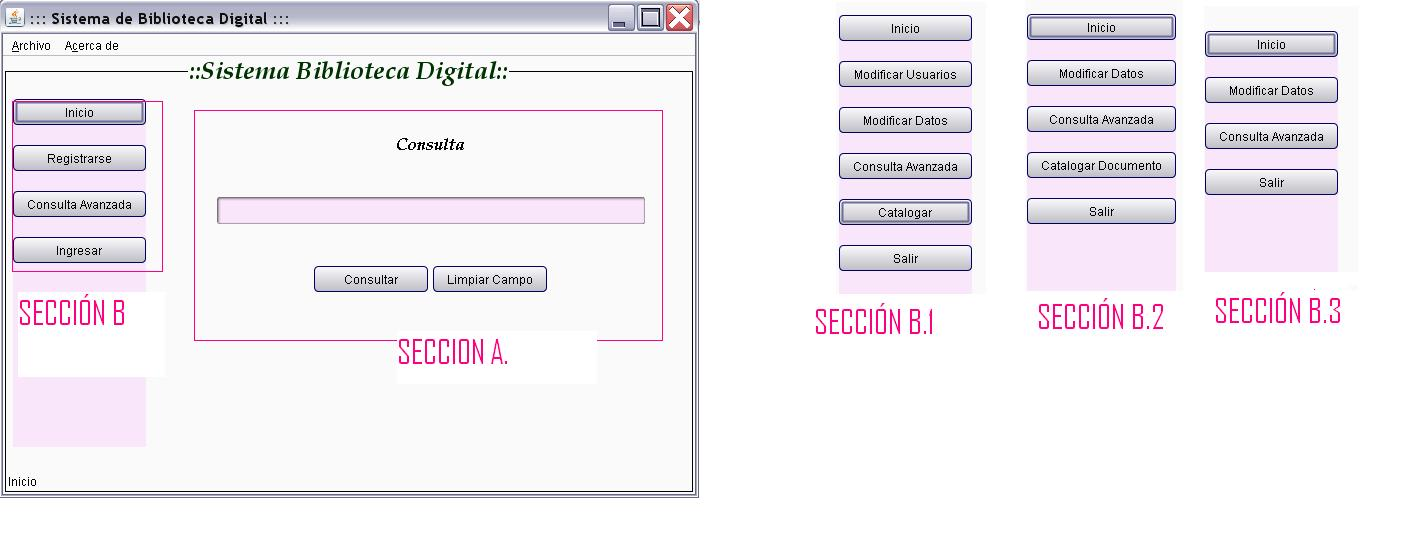
\includegraphics[width= 22cm , height= 13cm,angle=90]{Bocetos/guiPpal.jpg}
\caption{Boceto de la interfaz de inicio, la cual varia en su seccion B deacuerdo al perfil del usuario actualmente autentificado siendo seccion b.1 usuario administrador  , seccion B.2 usuario catalogardor , siendo seccion B.3 usuario normal. }
\end{figure}

\begin{figure}[h]
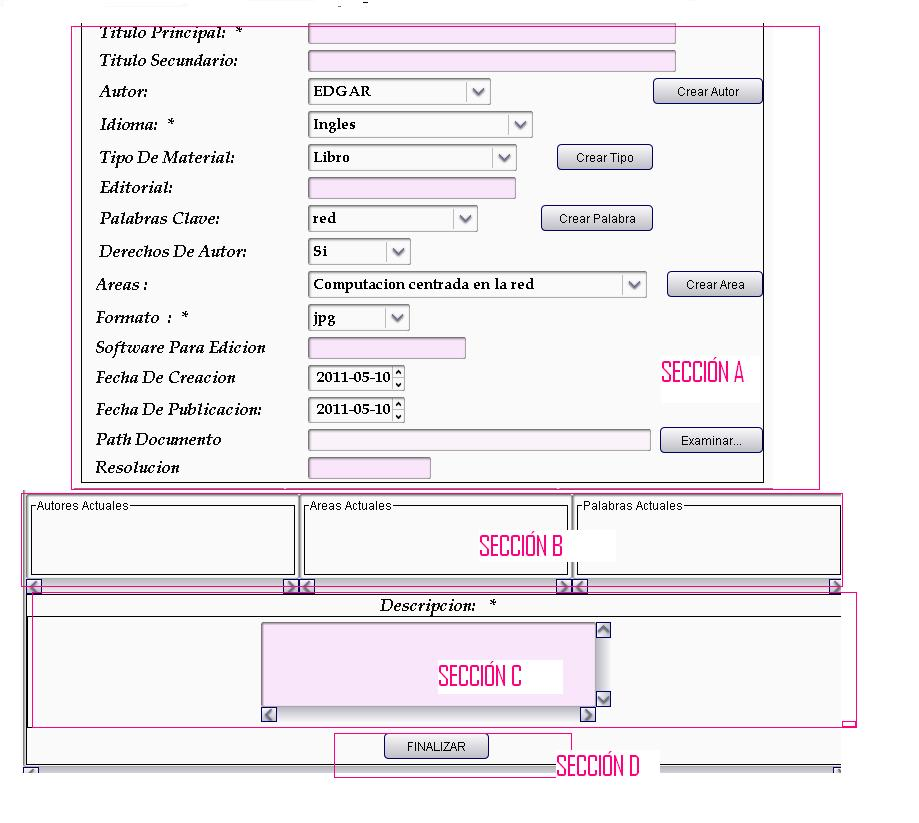
\includegraphics[width= 18cm , height= 15cm]{Bocetos/catalogarDoc.jpg}
\caption{Boceto de la interfaz de catalogar documento la cual permite añadir nuevos documento a la base de datos con ciertos metadatos ya especificados. }
\end{figure}

\begin{figure}[h]
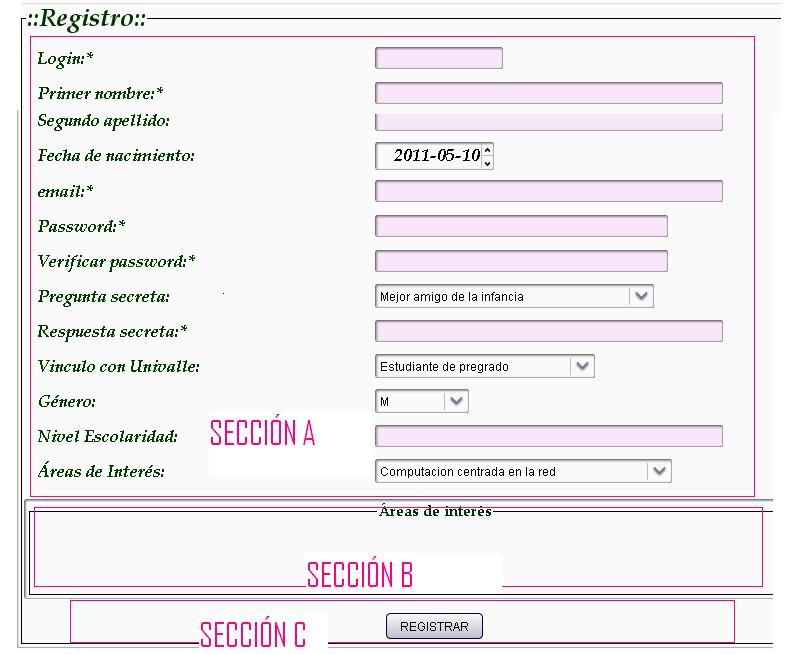
\includegraphics[width= 18cm , height= 13cm]{Bocetos/registro.jpg}
\caption{Boceto de la interfaz de registro de usuarios mediante la cual ingresa sus datos el usuario para pertenecer a la base de datos . }
\end{figure}

\begin{figure}[h]
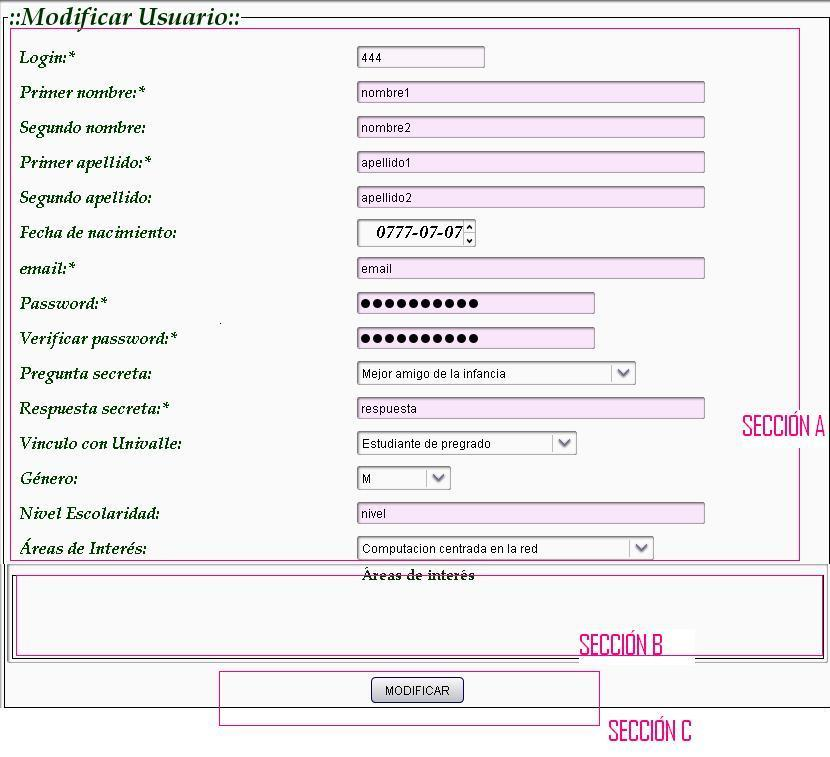
\includegraphics[width= 18cm , height= 13cm]{Bocetos/modificarUsuarios.jpg}
\caption{Boceto de la interfaz de modificar datos de usuarios la cual me permite modificar solo algunos datos del usuario activo. }
\end{figure}

\begin{figure}[h]
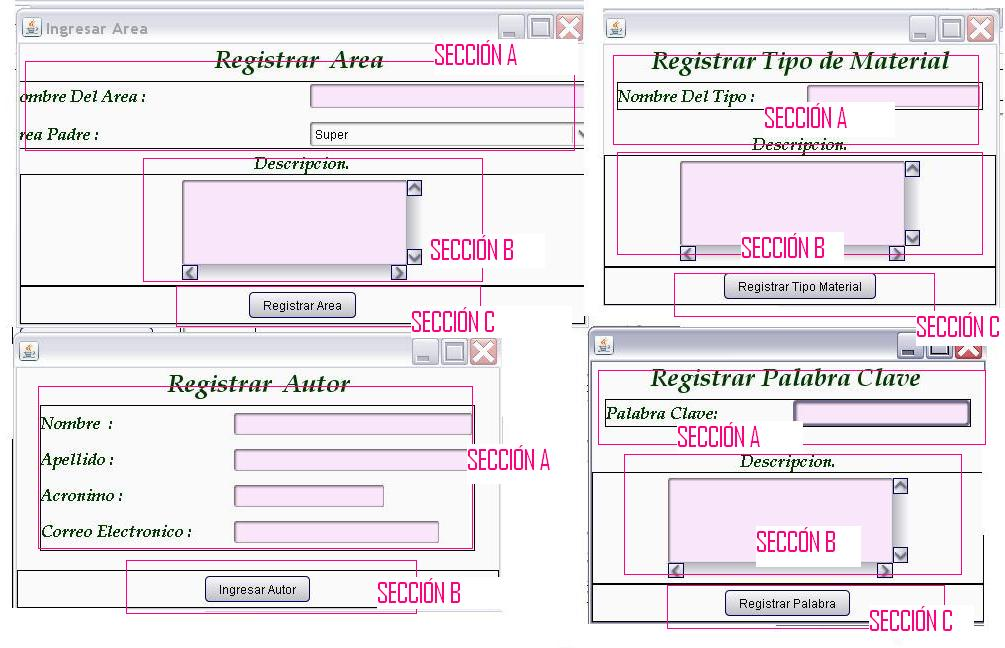
\includegraphics[width= 18cm , height= 13cm]{Bocetos/gestionDocumento.JPG}
\caption{Boceto de la interfaces de lo que tiene que ver con la gestion de documento ingresar un nuevo autor palabra clave tipo material y area al a que pertenece el documento. }
\end{figure}
\end{document}